\section{速度的瞬时性}\label{sec:01.06}

机械运动的现象,给了我们对“快”、“慢”的经验认识。
火车比轮船快,飞机比火车快,而火箭更比飞机快等等。反映质
点运动快慢的物理量就是速度,或者确切地说,是速度的数值大小。

先以直线运动为例,当时刻$ t_1 $时,质点$ A $的位置坐标为$ x\left(t_1\right) $,
当$ t_2 $时,它的坐标为$ x\left(t_2\right) $,我们就用下式来定义质点$ A $在$ t_1 $到
$ t_2 $时间间隔内的平均速度:
\begin{equation}
 \langle v\rangle_{t_{1} \rightarrow t_{2}}=\frac{x\left(t_{2}\right)-x\left(t_{1}\right)}{t_{2}-t_{1}} \label{eqn:01.06.01}
\end{equation}
符号$\langle ~ \rangle$表示所讨论的量的平均值。$\langle v\rangle_{t_{1} \rightarrow t_{2}}$的数值表示质点
在时
\clearpage
\noindent 间间隔$t_{1} \rightarrow t_{2}$中每单位时同平均走过的距离,它的单位是
米/秒。利用表\ref{tab:01.04}所给出的运动进行计算,就有:在第1秒末到
第2秒末间隔中,
\begin{equation*}
 \langle v\rangle_{1 \rightarrow 2}=\frac{34-17}{2-1}=17\,\text{米/秒}
\end{equation*}
在第3秒末到第5秒末间隔中,
\begin{equation*}
 \langle v\rangle_{3 \rightarrow 5}=\frac{85-51}{5-3}=17\,\text{米/秒}
\end{equation*}
选两个时间间隔中平均速度是一样的。事实上,如果利用分析表
达式\eqref{eqn:01.05.01}~来计算,就会发现对任何时间间隔,运动的平均速度
都是17米/秒。这种对于任何时间间隔平均速度总不变的运动,称
为匀速直线运动。

由表\ref{tab:01.05}~或$x=4.9t^2$所示的自由落体运动,情况就不同了:
在第1秒末到第3秒束的问隔中,
\begin{equation*}
 \langle v\rangle_{1 \rightarrow 3}=\frac{44.1-4.9}{3-1}=19.6\,\text{米/秒}
\end{equation*}
在第1秒末到第2秒末的间隔中,
\begin{equation*}
 \langle v\rangle_{1 \rightarrow 2}=\frac{19.6-4.9}{2-1}=14.7\,\text{米/秒}
\end{equation*}
在第2秒末到第3秒末的间隔中,
\begin{equation*}
 \langle v\rangle_{2 \rightarrow 3}=\frac{44.1-19.6}{3-2}=25.4\,\text{米/秒}
\end{equation*}
对于不同的时间间隔。自由落体的平均速度不相同。这种运动称
为变速运动。从上面所给出的三个平均速度可知,自由落体在第
1秒末到第3秒末的两秒钟时间间隔中并非匀速,它在前一秒钟
(即第1秒末到第2秒末)平均速度较小,在后一秒钟(即第2秒末
到第3秒末)平均速度较大。从这一点上可以充分反映出平均速度
往往不足以描写变速运动的细致情况。这是平均速度概
念的弱点。求平均速度的时间间隔取得越大,它对快慢的描述就越粗略;
反之,时间间隔越小,对快慢的描述也就越精确。在上例中,虽
然取1秒的时间间隔,比取2秒的时间间隔要好一些,但是在一
秒钟的时间间隔内,自由落体仍然不是匀速的。这种情况迫使我
们把计算平均速度的时间间隔取得尽可能地小。

为了便于进一步讨论,我们将式\ref{eqn:01.06.01}~中的
$t_2$表示成$t_2=t_1+\Delta t$,这个$\Delta t$就是求平均速
度所选用的时间间隔。现在来求从第1秒末到第$1+\Delta t$秒末
的间隔中,自由落体的平均速度。利用$x=4.9t^2$得到
\begin{equation*}
 \begin{aligned}
 \langle v\rangle_{1 \rightarrow 1+\Delta t} & =\frac{x\left(1+\Delta t\right)-x\left(1\right)}{1+\Delta t-1} \\
 & =\frac{4.9 \times\left(1+\Delta t\right)^{2}-4.9 \times 1^{2}}{\Delta t} \\
 & =\left(9.8+4.9 \Delta t\right) \text { 米/秒 }
 \end{aligned}
\end{equation*}
此式再次表明,从第1秒末开始取不同的时间间隔$\Delta t$,所得的平
均速度是不相同的。既然$\Delta t$越小描述得越精确,我们取
$\Delta t$为无限小,或者相当于$\Delta t \rightarrow 0$的
极限情况,这时平均速度变成为:
\begin{equation*}
 \lim _{\Delta t \rightarrow 0}\left(9.8+4.9 \Delta t\right)=9.8 \text { 米/秒 }
\end{equation*}
这个9.8米/秒的物理意义是自由落体在第1秒末的一个无限小时
间间隔中的平均速度,我们称这个值为自由落体在第1秒末的瞬
时速度。瞬时速度与平均速度这两个概念的重要区别在于:平均
速度总是与一段有限的时间间隔相联系,它是描述一段运动过程
的物理量;相反,瞬时速度与一个时刻相联系,它是描述运动的
瞬时性质的物理量。有了瞬时速度这个概念,使我们对运动的认
识大为深化。

用类似的手续不难求出自由落体运动在任何时刻t的瞬时速
度$v\left(t\right)$,只要将上述的1及$1+\Delta t$分别代之以$t$及$t+\Delta t$,并取
于$\Delta t \rightarrow 0$的极限值就可以了。故有

\begin{equation}\label{eqn:01.06.02}
 \begin{aligned}
 v\left(t\right) & =\lim _{\Delta t \rightarrow 0} \frac{x\left(t+\Delta t\right)-x\left(t\right)}{\Delta t} \\
 & =\lim _{\Delta t \rightarrow 0} \frac{4.9 \times\left(t+\Delta t\right)^{2}-4.9 \times t^{2}}{\Delta t} \\
 & =\lim _{\Delta t \rightarrow 0}\left(9.8 t+4.9 \Delta t\right) \\
 & =9.8 t
 \end{aligned}
\end{equation}
此式给出了自由落体在每个时刻的瞬时速度。根据这个结果,我
们再强调一遍,自由落体的运动快慢是时刻变化着的。你用平均
速度来描写它,无论$\Delta t$取如何小的有限值,即使小到$\Delta t$=0.001
秒,依然不够精确,因为在这0.001秒中质点依然不是匀速运动
的。只有$\Delta t$趋于无限小,给出了每个时刻$t$的瞬时速度,了解了
质点运动在每一瞬时的快慢,才算最精确地反映了质点运动的快
慢。

对于任何直线运动,它的瞬时速度都可以用类似方式来确
定:
\begin{equation*}
 v\left(t\right)=\lim _{\Delta t \rightarrow 0} \frac{x\left(t+\Delta t\right)-x\left(t\right)}{\Delta t}
\end{equation*}
根据微积分学的知识,该极限就是轨迹函数$x\left(t\right)$对时间t的一阶
导数。即
\begin{equation}
 \begin{aligned}
 v\left(t\right) & =\lim _{\Delta t \rightarrow 0} \frac{x\left(t+\Delta t\right)-x\left(t\right)}{\Delta t} \\
 & =\lim _{\Delta t \rightarrow 0} \frac{\Delta x}{\Delta t}=\frac{\dif x}{\dif t} \label{eqn:01.06.03}
 \end{aligned}
\end{equation}
其中,$\Delta x=x\left(t+\Delta t\right)-x\left(t\right)$,是在$t\rightarrow t+\Delta t$时间间隔中质点位置
坐标的增量。以后我们提到的速度,一般都指瞬时速度。

我们看到,瞬时速度是利用数学上的微分概念来描写的。其
实,在历史上,正是由于牛顿在处理这类基本力学问题时需要一
种适当的数学工具,从而促使他创建了微积分学。这不仅使物理
概念得以准确地表述,而且也大大丰富了数学本身。这是牛顿的
巨大功绩之一。\ziju{-0.02}由此,我们再次看到,一个物理对象,用什么数学
语言描写并不是一件自然的事情,而是物理研究的一个核心课题。\ziju{0}

\begin{wrapfigure}[10]{r}{13em}
 \centering
 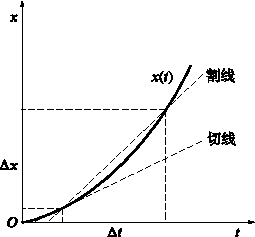
\includegraphics{figure/fig01.10}
 \caption{直线运动的$x \mathdash t$图}
 \label{fig:01.10}
\end{wrapfigure}
当质点作直线运动时,我们
可以设法求出它的位置时间曲线
(图\ref{fig:01.10})。从图中可以看出,平
均速度在数值上等于各段割线的
斜率,瞬时速度在数值上等于各
点的切线的斜率。所以在求出位
置时间曲线后,就可以从$x\left(t\right)$曲
线上求出各点的速度。

从平均速度的定义(\ref{eqn:01.06.01})式可以知道,$\langle v\rangle$可以有正值,
也可以有负值。当$x\left(t+\Delta t\right)<x\left(t\right)$时,$\langle v\rangle$为负。这种情况相当
于质点在$t$到$t+\Delta t$间隔中,总的说来是向负$x$方向运动的。所
以,$\langle v\rangle$的正负恰恰反映了运动的方向。通常称平均速度的绝对
值$|\langle v\rangle|$为平均速率。类似地,瞬时速度的绝对值$|\vec{v}\left(t\right)|$被称为
速率,而瞬时速度的正负,就表示质点在时刻$t$的运动方向。速
度$\vec{v}$不仅描述了运动的快慢,而且描述了运动方向。